\chapter{Sampling and Time-Discrete Signals and Systems}

\begin{refsection}

\section{Time-Discrete Signals}

\subsection{Ideal Sampling}

\begin{figure}[H]
	\centering
	\begin{tikzpicture}
		\begin{axis}[
			height={0.25\textheight},
			width=0.6\linewidth,
			scale only axis,
			xlabel={$t$},
			ylabel={$x$},
			%grid style={line width=.6pt, color=lightgray},
			%grid=both,
			grid=none,
			legend pos=north west,
			axis y line=middle,
			axis x line=middle,
			every axis x label/.style={
				at={(ticklabel* cs:1.05)},
				anchor=north,
			},
			every axis y label/.style={
				at={(ticklabel* cs:1.05)},
				anchor=east,
			},
			%xmin=0,
			%xmax=7,
			%ymin=0,
			%ymax=3,
			%xtick={0, 1, ..., 6},
			%ytick={0, 0.5, ..., 2.5},
			xmin=0,
			xmax=6.5,
			xtick={0, 1, ..., 6},
			xticklabels={$0$, $T_S$, $2 T_S$, $3 T_S$, $4 T_S$, $5 T_S$, $6 T_S$},
		]
			\addplot[smooth, blue, dashed] coordinates {(0, 1.1) (1, 1.8) (2, 2.1) (3, 1.0) (4, 0.8) (5, 1.7) (6, 2.4)};
			\addlegendentry{$\underline{x}{t}$};
			\addplot[red, thick] coordinates {(0, 0) (0, 1.1)};
			\addplot[red, thick] coordinates {(1, 0) (1, 1.8)};
			\addplot[red, thick] coordinates {(2, 0) (2, 2.1)};
			\addplot[red, thick] coordinates {(3, 0) (3, 1.0)};
			\addplot[red, thick] coordinates {(4, 0) (4, 0.8)};
			\addplot[red, thick] coordinates {(5, 0) (5, 1.7)};
			\addplot[red, thick] coordinates {(6, 0) (6, 2.4)};
			\addplot[only marks, red, thick, mark=o] coordinates {(0, 1.1) (1, 1.8) (2, 2.1) (3, 1.0) (4, 0.8) (5, 1.7) (6, 2.4)};
			\addlegendentry{$\underline{x}_S{t}$};
		\end{axis}
	\end{tikzpicture}
	\caption{Sampling of a time-continuous signal}
	\label{fig:ch04:sampling_of_signal}
\end{figure}

Sampling:
\begin{itemize}
	\item Sampling is converting a time-continuous signal $\underline{x}(t)$ to a time-discrete signal $\underline{x}[n]$.
	\item Samples are periodically taken out of the original signal.
\end{itemize}

Nomenclature:
\begin{itemize}
	\item The original time-continuous signal is $\underline{x}(t)$. The continuous time variable $t \in \mathbb{R}$ is a continuous real number.
	\item The sampled signal is $\underline{x}[n]$. The discrete time variable $n \in \mathbb{Z}$ is a (discrete) integer number.
	\item Round parenthesis is used for time-continuous signals. Square parenthesis is used for time-discrete signals.
\end{itemize}

Sampling parameters:
\begin{itemize}
	\item The time instances, at which the samples are taken out, are equidistant.
	\item The period between the samples is the \index{sampling period} \textbf{sampling period} $T_S$.
	\item The inverse of the sampling period is the \index{sampling rate} \textbf{sampling rate} $f_S$.
	\begin{equation}
		f_S = \frac{1}{T_S}
	\end{equation}
	\item The \index{sampling angular frequency} \textbf{sampling angular frequency} $\omega_S$.
	\begin{equation}
		\omega_S = \frac{2 \pi}{T_S}
	\end{equation}
\end{itemize}

Ideal sampling:
\begin{itemize}
	\item The samples are ideally equidistant. The sampling period $T_S$ is constant and is \underline{not} subject to fluctuations.
	\item The sample has the value of the original signal $\underline{x}(t)$ at \underline{exactly} the time instance where has been taken.
\end{itemize}
Some corollaries can be deducted from these two points:
\begin{itemize}
	\item The sampled signal $\underline{x}_S(n T_S)$ at the discrete time $n$ is the value of the original signal at time $t = n T_S$.
	\begin{equation}
		\underline{x}[n] = \underline{x}\left(n T_S\right)
	\end{equation}
	\item The sampled signal $\underline{x}_S(t)$ consists of a chain of equidistant, indefinitely narrow pulses.
	\begin{itemize}
		\item The pulses are equidistant with $T_S$.
		\item The pulses have the value of $\underline{x}\left(n T_S\right)$ as their amplitudes.
		\item The value of the sampled signal is zero in between the pulses.
		\begin{equation}
			\underline{x}_S(t) = \begin{cases}
				\underline{x}\left(n T_S\right) & \quad \forall \; t = n T_S, n \in \mathbb{Z}, \\
				0 & \quad \forall \; n T_S < t < \left(n+1\right) T_S, n \in \mathbb{Z}.
			\end{cases}
		\end{equation}
	\end{itemize}
\end{itemize}

We know already indefinitely narrow pulses. They are Dirac delta functions $\delta\left(t - n T_S\right)$.

Taking out \underline{exactly one} sample out of $\underline{x}(t)$ is a multiplication of $\underline{x}(t)$ with $\delta\left(t - n T_S\right)$.
\begin{equation}
	\underline{x}_{S,n}(t) = \underline{x}(t) \delta\left(t - n T_S\right)
	\label{eq:ch4:one_sample_1}
\end{equation}
The Dirac delta function is zero expect at $t = n T_S$. So, \eqref{eq:ch4:one_sample_1} can be further reduced.
\begin{equation}
	\underline{x}_{S,n}(t) = \underline{x}(n T_S) \delta\left(t - n T_S\right)
	\label{eq:ch4:one_sample_2}
\end{equation}

\begin{figure}[H]
	\centering
	\begin{tikzpicture}
		\begin{axis}[
			height={0.25\textheight},
			width=0.6\linewidth,
			scale only axis,
			xlabel={$t$},
			ylabel={$x$},
			%grid style={line width=.6pt, color=lightgray},
			%grid=both,
			grid=none,
			legend pos=north west,
			axis y line=middle,
			axis x line=middle,
			every axis x label/.style={
				at={(ticklabel* cs:1.05)},
				anchor=north,
			},
			every axis y label/.style={
				at={(ticklabel* cs:1.05)},
				anchor=east,
			},
			%xmin=0,
			%xmax=7,
			%ymin=0,
			%ymax=3,
			%xtick={0, 1, ..., 6},
			%ytick={0, 0.5, ..., 2.5},
			xmin=0,
			xmax=6.5,
			xtick={0, 1, ..., 6},
			xticklabels={$0$, $T_S$, $2 T_S$, $3 T_S$, $4 T_S$, $5 T_S$, $6 T_S$},
		]
			\addplot[smooth, blue, dashed] coordinates {(0, 1.1) (1, 1.8) (2, 2.1) (3, 1.0) (4, 0.8) (5, 1.7) (6, 2.4)};
			\addlegendentry{$\underline{x}{t}$};
			\addplot[red, thick] coordinates {(2, 0) (2, 2.1)};
			\addplot[only marks, red, thick, mark=o] coordinates {(2, 2.1)};
			\addlegendentry{$\underline{x}_{S,n}{t}$};
		\end{axis}
	\end{tikzpicture}
	\caption[Taking out exactly one sample out of $\underline{x}(t)$]{Taking out exactly one sample out of $\underline{x}(t)$ -- in this example $n = 2$.}
\end{figure}

To obtain the sampled signal, the sampling process $\underline{x}_{S,n}(t)$ \eqref{eq:ch4:one_sample_1} needs to be repeated for each $n \in \mathbb{Z}$. All individual sample processes $\underline{x}_{S,n}(t)$ are then superimposed to form the complete sampled signal $\underline{x}_S(t)$.
\begin{equation}
	\begin{split}
		\underline{x}_S(t) &= \sum\limits_{n = -\infty}^{\infty} \underline{x}_{S,n}(t) \\
		 &= \sum\limits_{n = -\infty}^{\infty} \underline{x}\left(t\right) \delta\left(t - n T_S\right) \\
		 &= \underline{x}\left(t\right) \cdot \underbrace{\sum\limits_{n = -\infty}^{\infty} \delta\left(t - n T_S\right)}_{= \Sha_{T_S}(t)}
	\end{split}
\end{equation}

The sum of Dirac delta functions
\begin{itemize}
	\item forms a series of equidistant pulses repeating at a period of $T_S$,
	\item is called \index{Dirac comb} \textbf{Dirac comb} $\Sha_{T_S}(t)$ or \index{impulse train} \textbf{impulse train}.
\end{itemize}

\begin{equation}
	\Sha_{T_S}(t) = \sum\limits_{n = -\infty}^{\infty} \delta\left(t - n T_S\right)
\end{equation}
\begin{figure}[H]
	\centering
	\begin{tikzpicture}
		\begin{axis}[
			height={0.15\textheight},
			width=0.9\linewidth,
			scale only axis,
			xlabel={$t$},
			ylabel={$\Sha_{T_S}(t)$},
			%grid style={line width=.6pt, color=lightgray},
			%grid=both,
			grid=none,
			legend pos=north east,
			axis y line=middle,
			axis x line=middle,
			every axis x label/.style={
				at={(ticklabel* cs:1.05)},
				anchor=north,
			},
			every axis y label/.style={
				at={(ticklabel* cs:1.05)},
				anchor=east,
			},
			xmin=-5.5,
			xmax=5.5,
			ymin=0,
			ymax=1.2,
			xtick={-5, -4, ..., 5},
			xticklabels={$-5 T_S$, $-4 T_S$, $-3 T_S$, $-2 T_S$, $- T_S$, $0$, $T_S$, $2 T_S$, $3 T_S$, $4 T_S$, $5 T_S$},
			ytick={0},
		]
			\pgfplotsinvokeforeach{-5, -4, ..., 5}{
				\draw[-latex, blue, very thick] (axis cs:#1,0) -- (axis cs:#1,1);
				%\addplot[blue, very thick] coordinates {(#1, 0) (#1, 1)};
				%\addplot[only marks, blue, thick, mark=triangle] coordinates {(#1, 1)};
			}
		\end{axis}
	\end{tikzpicture}
	\caption{Dirac comb}
\end{figure}

A \index{sampler} \textbf{sampler} is a system which
\begin{itemize}
	\item applies the Dirac comb $\Sha_{T_S}(t)$
	\item to a time-continuous signal $\underline{x}(t)$ (multiplication) and
	\item outputs a series of equidistant pulses $\underline{x}_S(t)$.
\end{itemize}
\begin{equation}
	\begin{split}
		\underline{x}_S(t) &= \underline{x}(t) \cdot \Sha_{T_S}(t) \\
		 &= \sum\limits_{n = -\infty}^{\infty} \underline{x}\left(t\right) \delta\left(t - n T_S\right) \\
		 &= \sum\limits_{n = -\infty}^{\infty} \underline{x}\left(n T_S\right) \delta\left(t - n T_S\right)
	\end{split}
	\label{eq:ch04:ideal_sampling}
\end{equation}

The sampled signal $\underline{x}_S(t)$ is a chain of pulses (red signal in Figure \ref{fig:ch04:sampling_of_signal}). The chain of pulses can then be reinterpreted as a time-discrete signal $\underline{x}[n]$. The value of $\underline{x}[n]$ is:
\begin{equation}
	\underline{x}[n] = \underline{x}_S\left(n T_S\right) = \underline{x}\left(n T_S\right) \qquad \forall \; n \in \mathbb{Z}
	\label{eq:ch04:sample_value}
\end{equation}

\begin{figure}[H]
	\centering
	\begin{adjustbox}{scale=0.8}
		\begin{tikzpicture}
			\node[draw, block] (Sampler) {Ideal sampler};
			\node[draw, block, right=3cm of Sampler] (ReInterp) {Reinterpret as\\ time-discrete signal};
			
			\draw[<-o] (Sampler.west) -- ++(-1.7cm, 0) node[above, align=center]{Time-continuous\\ signal $\underline{x}(t)$};
			\draw[->] (Sampler.east) -- (ReInterp.west) node[midway, above, align=center]{Series of pulses\\ $\underline{x}_S(t)$};
			\draw[<-] (Sampler.south) -- ++(0, -0.75cm) node[below, align=center]{Dirac comb\\ $\Sha_{T_S}(t)$};
			\draw[->] (ReInterp.east) -- ++(1.5cm, 0) node[above, align=center]{Time-discrete\\ signal $\underline{x}[n]$};
			
			\draw[dashed] (ReInterp.north) -- ++(0, 2cm) node[below left, align=right]{Time-continuous\\ domain} node[below right, align=left]{Time-discrete\\ domain};
			\draw[dashed] (ReInterp.south) -- ++(0, -1cm);
		\end{tikzpicture}
	\end{adjustbox}
	\caption{An abstract view on sampling}
\end{figure}

\begin{fact}
	The act of sampling is irreversible.
\end{fact}
	
There is a way to obtain the sampled signal:
\begin{equation*}
	\underline{x}_S(t) = \mathrm{Sampling} \left(\underline{x}(t)\right)
\end{equation*}
But there is generally no way back to reconstruct the original signal. $\mathrm{Sampling}^{-1} \left(\underline{x}_S(t)\right)$ does not exist.
\begin{equation*}
	\underline{x}(t) \neq \underbrace{\mathrm{Sampling}^{-1}}_{\text{Does not exist}} \left(\underline{x}_S(t)\right)
\end{equation*}

Sampling is always lossy in general.

\subsection{Sampling Theorem and Aliasing}


\subsection{Discrete-Time Fourier Transform}

% TODO
Using \eqref{eq:ch04:ideal_sampling} and \eqref{eq:ch04:sample_value}, a expression depending on the time-discrete signal $\underline{x}[n]$ can be formulated:
\begin{equation}
	\underline{x}_S(t) = \sum\limits_{n = -\infty}^{\infty} \underline{x}[n] \cdot \delta(t - n T_S)
\end{equation}

The Fourier transform of the sampled signal $\underline{x}_S(t)$ is:
\begin{equation}
	\begin{split}
		\underline{X}_S \left(j \omega\right) &= \mathcal{F} \left\{\underline{x}_S(t)\right\} \\
		 &= \mathcal{F} \left\{\sum\limits_{n = -\infty}^{\infty} \underline{x}[n] \cdot \delta(t - n T_S)\right\} \\
		 &= \int\limits_{t = -\infty}^{\infty} \sum\limits_{n = -\infty}^{\infty} \underline{x}[n] \cdot \delta(t - n T_S) \cdot e^{-j \omega t} \, \mathrm{d} t \\
		 &= \sum\limits_{n = -\infty}^{\infty} \int\limits_{t = -\infty}^{\infty} \underline{x}[n] \cdot \delta(t - n T_S) \cdot e^{-j \omega t} \, \mathrm{d} t \\
		 &= \sum\limits_{n = -\infty}^{\infty} \underline{x}[n] \cdot e^{-j \omega n T_S}
	\end{split}
\end{equation}

Redefining $\phi = T_S \omega$:
\begin{equation}
	\underline{X}_S \left(j \omega\right) = \underline{X} \left(e^{j \phi}\right) = \sum\limits_{n = -\infty}^{\infty} \underline{x}[n] \cdot e^{-j \phi n}
\end{equation}

\subsection{Discrete Fourier Transform}

\section{Analogies Of Time-Continuous and Time-Discrete Signals and Systems}

\subsection{Transforms}

\begin{table}[H]
	\centering
	\begin{tabular}{|p{0.3\linewidth}||p{0.3\linewidth}|p{0.3\linewidth}|}
		\hline
		{} & \textbf{Frequency-Continuous Domain} & \textbf{Frequency-Discrete Domain} \\
		\hline
		\hline
		\textbf{Time-Continuous Domain} & Fourier transform & Fourier series \\
		\hline
		\textbf{Time-Discrete Domain} & Discrete-Time Fourier transform & Discrete Fourier transform \\
		\hline
	\end{tabular}
\end{table}

\subsubsection{Obtaining a frequency-continuous domain:}

\begin{minipage}{0.45\linewidth}
	\textbf{From the time-continuous domain (analog signal):}
	
	\vspace{0.5em}
	
	Fourier transform:
	\begin{equation*}
		\underline{X}(j \omega) = \int\limits_{t = -\infty}^{\infty} \underline{x}(t) \cdot e^{-j \omega t} \, \mathrm{d} t
	\end{equation*}
	
	Inverse Fourier transform:
	\begin{equation*}
		\underline{x}(t) = \frac{1}{2 \pi} \int\limits_{\omega = -\infty}^{\infty} \underline{X}(j \omega) \cdot e^{+ j \omega t} \, \mathrm{d} \omega
	\end{equation*}
	
	\begin{itemize}
		\item Continuous time: $t \in \mathbb{R}$
		\item Continuous frequency: $\omega \in \mathbb{R}$
	\end{itemize}
\end{minipage}
\hfill
\begin{minipage}{0.45\linewidth}
	\textbf{From the time-discrete domain (digital signal):}
	
	\vspace{0.5em}
	
	Discrete-time Fourier transform:
	\begin{equation*}
		\underline{X}_{2\pi}(e^{j \phi}) = \sum\limits_{n = -\infty}^{\infty} \underline{x}[n] \cdot e^{- j \phi n}
	\end{equation*}
	
	Inverse discrete-time Fourier transform:
	\begin{equation*}
		\underline{x}[n] = \frac{1}{2 \pi} \int\limits_{- \pi}^{+ \pi} \underline{X}_{2\pi}(e^{j \phi}) \cdot e^{+ j \phi n} \, \mathrm{d} \phi
	\end{equation*}
	
	\begin{itemize}
		\item Discrete time: $n \in \mathbb{Z}$
		\item Continuous frequency: $\phi \in \mathbb{R}$
	\end{itemize}
\end{minipage}

\subsubsection{Obtaining a frequency-discrete domain:}

\begin{minipage}{0.45\linewidth}
	\textbf{From the time-continuous domain (analog signal):}
	
	\vspace{0.5em}
	
	Fourier analysis:
	\begin{equation*}
		\underline{X}[k] = \frac{\omega_0}{2 \pi} \int\limits_{-\frac{T_0}{2}}^{\frac{T_0}{2}} \underline{x}(t) \cdot e^{-j k \omega_0 t} \, \mathrm{d} t
	\end{equation*}
	
	Fourier series:
	\begin{equation*}
		\underline{x}(t) = \sum\limits_{k = -\infty}^{\infty} \underline{X}[k] \cdot e^{+ j k \omega_0 t}
	\end{equation*}
	
	\begin{itemize}
		\item Continuous time: $t \in \mathbb{R}$
		\item Discrete frequency: $k \in \mathbb{Z}$
	\end{itemize}
\end{minipage}
\hfill
\begin{minipage}{0.45\linewidth}
	\textbf{From the time-discrete domain (digital signal):}
	
	\vspace{0.5em}
	
	Discrete Fourier transform:
	\begin{equation*}
		\underline{X}[k] = \sum\limits_{n = 0}^{N - 1} \underline{x}[n] \cdot e^{- j \frac{2 \pi}{N} k n}
	\end{equation*}
	
	Inverse discrete Fourier transform:
	\begin{equation*}
		\underline{x}[n] = \frac{1}{N} \sum\limits_{k = 0}^{N - 1} \underline{X}[k]  \cdot e^{+ j \frac{2 \pi}{N} k n}
	\end{equation*}
	
	\begin{itemize}
		\item Discrete time: $n \in \mathbb{Z}$
		\item Discrete frequency: $k \in \mathbb{Z}$
	\end{itemize}
\end{minipage}

\subsection{Systems}

\subsection{Cross-Correlation and Autocorrelation}

\subsection{Spectral Density}

\subsection{Noise}

\section{Digital Signals and Systems}

\subsection{Quantization}

\subsection{Quantization Error}

\subsection{Window Filters}

\subsection{Time Recovery}

\subsection{Practical Issues}

\phantomsection
\addcontentsline{toc}{section}{References}
\printbibliography[heading=subbibliography]
\end{refsection}

